% Figure 3 — Leakage-free selection pipeline (20 candidates -> single DS03 test)
\documentclass[tikz,border=6pt]{standalone}
% Meta AI / FAIR figure style (I-JEPA / V-JEPA visual language)
% White background, soft pastel rounded blocks, thin borders, sans-serif,
% dashed arrows for EMA / stop-gradient, minimal ink.
\usepackage{amsmath,amssymb}
\usepackage[scaled]{helvet}
\renewcommand{\familydefault}{\sfdefault}
\usepackage{tikz}
\usetikzlibrary{arrows.meta,positioning,fit,calc,backgrounds}

% --- FAIR-like palette -------------------------------------------------------
\definecolor{mblue}{HTML}{BDD7EE}   \definecolor{mblueL}{HTML}{2E75B6}  % context / online encoder
\definecolor{mpink}{HTML}{F8CBAD}   \definecolor{mpinkL}{HTML}{ED7D31}  % target (EMA) encoder
\definecolor{mgreen}{HTML}{C6E0B4}  \definecolor{mgreenL}{HTML}{548235} % predictor
\definecolor{myell}{HTML}{FFE699}   \definecolor{myellL}{HTML}{BF9000}  % actions / conditioning
\definecolor{mgray}{HTML}{F2F2F2}   \definecolor{mgrayL}{HTML}{7F7F7F}  % latents / neutral
\definecolor{mred}{HTML}{F4B8B8}    \definecolor{mredL}{HTML}{C00000}   % loss / dead controls
\definecolor{ink}{HTML}{3B3B3B}

\tikzset{
  every node/.style={font=\sffamily},
  blk/.style={rounded corners=7pt, line width=0.7pt, minimum height=9mm,
              inner xsep=3mm, inner ysep=2mm, align=center, font=\sffamily\small},
  enc/.style ={blk, fill=mblue,  draw=mblueL},
  tgt/.style ={blk, fill=mpink,  draw=mpinkL},
  prd/.style ={blk, fill=mgreen, draw=mgreenL},
  act/.style ={blk, fill=myell,  draw=myellL},
  lat/.style ={blk, fill=mgray,  draw=mgrayL},
  los/.style ={circle, fill=mred, draw=mredL, line width=0.7pt, minimum size=7.5mm,
               font=\sffamily\small, inner sep=0pt},
  lbl/.style ={font=\sffamily\footnotesize, text=ink},
  sub/.style ={font=\sffamily\scriptsize, text=mgrayL},
  ar/.style  ={-{Latex[length=2.4mm]}, line width=0.8pt, draw=ink},
  ema/.style ={-{Latex[length=2.4mm]}, line width=0.8pt, draw=mpinkL, dashed},
  sg/.style  ={ar, postaction={decorate}},  % stop-gradient: annotate with // manually
  cell/.style={draw=mgrayL, line width=0.4pt, minimum size=3.2mm, inner sep=0pt},
  cellm/.style={cell, fill=mblue},          % visible patch
  cellx/.style={cell, fill=mgray},          % masked patch
}
% stop-gradient tick: \sgmark{point}
\newcommand{\sgmark}[1]{\node[rotate=65, font=\footnotesize\bfseries, text=ink] at (#1) {/\!/};}

\begin{document}
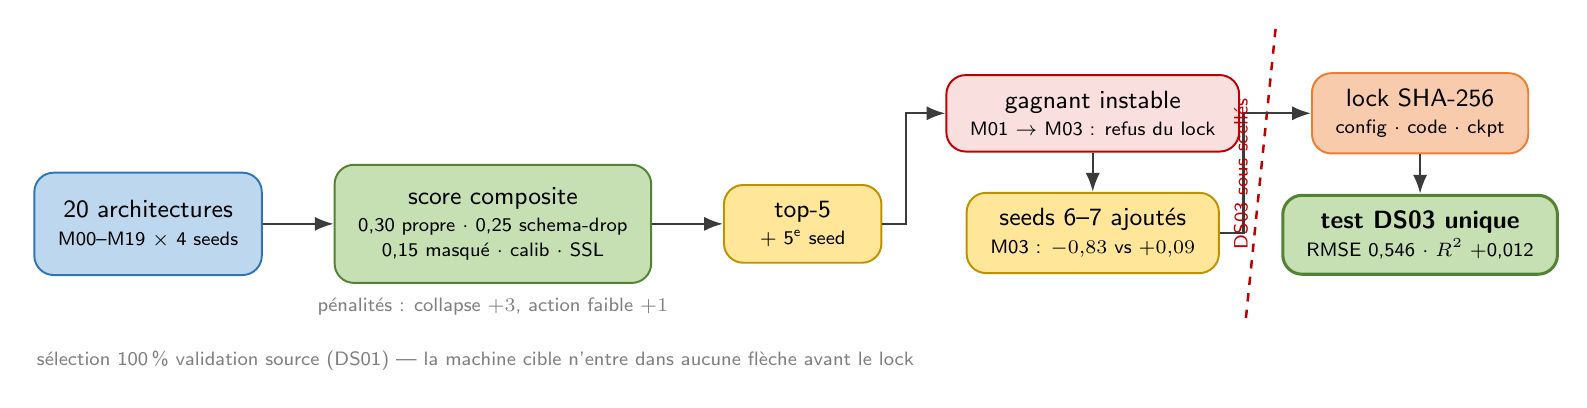
\begin{tikzpicture}[node distance=7mm]

\node[enc, minimum width=27mm, minimum height=13mm, align=center] (cand)
  {20 architectures\\[-1pt]{\scriptsize M00--M19 $\times$ 4 seeds}};

\node[prd, minimum width=30mm, minimum height=15mm, right=9mm of cand, align=center] (score)
  {score composite\\[-1pt]{\scriptsize 0{,}30 propre $\cdot$ 0{,}25 schema-drop}\\[-2pt]
   {\scriptsize 0{,}15 masqu\'e $\cdot$ calib $\cdot$ SSL}};
\node[sub, below=0.5mm of score] {p\'enalit\'es : collapse $+3$, action faible $+1$};

\node[act, minimum width=20mm, right=9mm of score, align=center] (top5)
  {top-5\\[-1pt]{\scriptsize $+$ 5\textsuperscript{e} seed}};

\node[blk, fill=mred!45, draw=mredL, minimum width=27mm, above right=4mm and 8mm of top5, align=center] (unst)
  {gagnant instable\\[-1pt]{\scriptsize M01 $\to$ M03 : refus du lock}};
\node[blk, fill=myell, draw=myellL, minimum width=27mm, below=5mm of unst, align=center] (more)
  {seeds 6--7 ajout\'es\\[-1pt]{\scriptsize M03 : $-0{,}83$ vs $+0{,}09$}};

\node[tgt, minimum width=25mm, right=9mm of unst, align=center] (lock)
  {lock SHA-256\\[-1pt]{\scriptsize config $\cdot$ code $\cdot$ ckpt}};
\node[blk, fill=mgreen, draw=mgreenL, line width=1.1pt, minimum width=25mm, below=5mm of lock, align=center] (test)
  {\textbf{test DS03 unique}\\[-1pt]{\scriptsize RMSE 0{,}546 $\cdot$ $R^2$ $+$0{,}012}};

\draw[ar] (cand) -- (score);
\draw[ar] (score) -- (top5);
\draw[ar] (top5.east) -- ++(3mm,0) |- (unst.west);
\draw[ar] (unst) -- (more);
\draw[ar] (more.east) -- ++(3mm,0) |- (lock.west);
\draw[ar] (lock) -- (test);

% the seal: DS03 never crosses this line
\begin{scope}[on background layer]
  \draw[dashed, line width=0.9pt, draw=mredL]
    ($(lock.north west)+(-0.45,0.55)$) -- ($(test.south west)+(-0.45,-0.55)$);
\end{scope}
\node[sub, text=mredL, rotate=90] at ($(lock.west)!0.5!(test.west)+(-0.7,0)$)
  {DS03 sous scell\'es};

\node[sub, align=center] at ($(cand.south)!0.5!(top5.south)+(0,-1.15)$)
  {s\'election 100\,\% validation source (DS01) --- la machine cible n'entre dans aucune fl\`eche avant le lock};

\end{tikzpicture}
\end{document}
